%%%%%%%%%%%%%%%%%%%%%%%%%%%%%%%%%%%%%%%%%%%%%%%%%%%%%%%%%%%%%%%%%%%%%%%%%%%%%%%% 
%                                   PREAMBLE                                   %
%%%%%%%%%%%%%%%%%%%%%%%%%%%%%%%%%%%%%%%%%%%%%%%%%%%%%%%%%%%%%%%%%%%%%%%%%%%%%%%% 

% Compile with 'latexmk -shell-escape -pdf guide'.

%%%% DOCUMENT CLASS %%%%%%%%%%%%%%%%%%%%%%%%%%%%%%%%%%%%%%%%%%%%%%%%%%%%%%%%%%%%

% Global options declared here may be used by packages below. For example:
%
% 1. Language options, like 'english' or 'spanish', are used by package 'babel'.
% 2. Paper size options, like 'a4paper', are used by package 'geometry'.
%
% Options like 'american', 'british', 'canadian', 'australian', 'newzealand'
% represent variants of English.

\documentclass[british,a4paper,11pt,titlepage]{article}

%%%% FONT ENCODING %%%%%%%%%%%%%%%%%%%%%%%%%%%%%%%%%%%%%%%%%%%%%%%%%%%%%%%%%%%%%

% T1 is an 8-bit encoding for a set of 256 glyphs, the standard LaTeX glyph set
% that covers most European languages that use Latin alphabets.

\usepackage[T1]{fontenc}        % T1 font encoding.

%%%% FONTS %%%%%%%%%%%%%%%%%%%%%%%%%%%%%%%%%%%%%%%%%%%%%%%%%%%%%%%%%%%%%%%%%%%%%

% Fonts should match the specified font encoding. There are different packages
% providing different fonts with different encodings.

\usepackage{lmodern}            % Translation of Computer Modern into T1 fonts.

% Alternative T1 fonts based on the Adobe Utopia fonts:
%
% Utopia Regular, Utopia Italic, Utopia Bold, and Utopia Bold Italic 
%
% \usepackage{fourier}
%
% Alternative T1 fonts containing the whole LaTeX glyph set and matching fonts
% for mathematics:
%
% https://www.ctan.org/pkg/mathdesign
%
% \usepackage[utopia]{mathdesign}
% \usepackage[garamond]{mathdesign}
% \usepackage[charter]{mathdesign}

% Font selection is greatly simplified with XeLaTeX and LuaLaTeX, particularly
% thanks to the use of Unicode and support for Apple Advanced Typography (AAT),
% TrueType (TTF) and OpenType (OTF) fonts through the fontspec package (other
% relevant packages include unicode-math, mathspec, and fontsetup). 
%
% A catalogue of free fonts can be found here:
%
% https://tug.org/FontCatalogue

%%%% INPUT ENCODING %%%%%%%%%%%%%%%%%%%%%%%%%%%%%%%%%%%%%%%%%%%%%%%%%%%%%%%%%%%%

% The selected encoding must match the encoding the file is written. For
% example, if you are using a Unicode text editor and saving your documents with
% the typical UTF-8 encoding, you should use the following:

\usepackage[utf8]{inputenc}

% In fact, this is the default input encoding in recent versions, so you can
% omit this, though it will not hurt.

% Unicode character recognition: https://shapecatcher.com
% LaTeX symbol recognition:      https://detexify.kirelabs.org

% Other usual encodings:

% \usepackage[latin1]{inputenc}   % ISO 8859-1 encoding.
% \usepackage[latin9]{inputenc}   % ISO 8859-15 encoding (includes the € sign).

%%%% PAGE FORMAT %%%%%%%%%%%%%%%%%%%%%%%%%%%%%%%%%%%%%%%%%%%%%%%%%%%%%%%%%%%%%%%

% Page geometry, margins, etc.

\usepackage{geometry}

% Empty pages really empty, without page numbers and headings.

\usepackage{emptypage}

% Paragraphs without indentation and separated by vertical space.

\usepackage[parfill]{parskip}

% PDF metadata, hyperlinks, and bookmarks.

\usepackage[pdfusetitle,colorlinks,citecolor=magenta,linkcolor=blue]{hyperref}

% Improved bookmarks.

\usepackage{bookmark}

% Author blocks (name and affiliation).

\usepackage[auth-sc,blocks]{authblk}

% We found a problem here! Unfortunately, package 'authblk' interferes with the
% inner mechanism by which 'hyperref' provides author metadata (pdfauthor)
% thanks to the option 'pdfusetitle'. As a consequence, author metadata in the
% PDF remains empty. However, we are fortunate, because LaTeX is free,
% open-source, programmable and well-documented. The same with these LaTeX
% packages. No wonder we could study the package documentation (and even the
% source code when necessary) and patch the definition of the '\author' macro to
% fix it. Even better. We were able to find an almost working solution in the
% Internet (TeX Stack Exchange).

\usepackage{xpatch}             % Patching facilities.

\xpretocmd{\author}{\addauthor{#2}}{}{}

\newif\iffirstauthor            % New 'if'.
\firstauthortrue                % Initially, true.

\newcommand{\addauthor}[1]
{
  \iffirstauthor                  % First author?
    \newcommand{\hrauthor}{#1}    % The author name.
    \firstauthorfalse
  \else                           % Other authors?
  \xapptocmd{\hrauthor}{, #1}{}{} % A comma followed by the author name.
  \fi
}

%%%% BIBLIOGRAPHY %%%%%%%%%%%%%%%%%%%%%%%%%%%%%%%%%%%%%%%%%%%%%%%%%%%%%%%%%%%%%%

% The modern and powerful BibLaTeX, with the default Biber back-end (option
% 'backend=biber' is set by default).

\usepackage{csquotes}           % Context-sensitive quotations.
\usepackage{biblatex}

% Changing the style.

% Numeric (the default style), in citation order, with back-references.

% \usepackage[style=numeric,sorting=none,backref]{biblatex}

% Author-year, sorted by name-year-volume-title.

% \usepackage[style=authoryear,sorting=nyvt,block=space,backref]{biblatex}

% It is possible to mix styles (the combination should be sensible so that it
% does not hamper search in a printed copy). For example, author-year for
% citations and author-title for bibliography items.

% \usepackage[citestyle=authoryear,bibstyle=authortitle,block=ragged]{biblatex}

% Redefining the URL field (break the line before and turn the space after the
% colon into a non-breaking space 

\DeclareFieldFormat{url}{\newline\mkbibacro{URL}\addcolon\nobreakspace\url{#1}}

\addbibresource{references.bib}

%%%% MATHEMATICS %%%%%%%%%%%%%%%%%%%%%%%%%%%%%%%%%%%%%%%%%%%%%%%%%%%%%%%%%%%%%%%

% AMS mathematical delicatessen.

\usepackage{amsmath}
\usepackage{amssymb}
\usepackage{amsthm}

%%%% FIGURES AND TABLES %%%%%%%%%%%%%%%%%%%%%%%%%%%%%%%%%%%%%%%%%%%%%%%%%%%%%%%%

% Publication-quality tables.

\usepackage{array,booktabs}

% Captions for subfigures and subtables.
%
% This is an alternative to package subfig. Please, notice that package
% subfigure, which is superseded by subfig, is obsolete and deprecated.

\usepackage{subcaption}

% Enhanced support for the inclusion of external graphics.

\usepackage{graphicx}

% Plots and tables with TikZ & PGF.

\usepackage{pgfplotstable}

\usetikzlibrary{intersections}

%%%% CODE AND PSEUDO CODE FORMATTING %%%%%%%%%%%%%%%%%%%%%%%%%%%%%%%%%%%%%%%%%%%

% Improved verbatim text.

% \usepackage{verbatim}

% Much improved, and configurable, verbatim text.

% \usepackage{fancyvrb}

% Source code listing with basic syntax highlighting.

% \usepackage{listings}

% Syntax highlighting through Python's Pygments library.
%
% apt install python-pygments
%
% Please, notice that '-shell-escape' will be required when compiling to
% execute the necessary external commands.

\usepackage[cachedir=.minted-\jobname]{minted}

%%%% ATTACHMENTS %%%%%%%%%%%%%%%%%%%%%%%%%%%%%%%%%%%%%%%%%%%%%%%%%%%%%%%%%%%%%%%

% Attach source files to the output PDF document.

\usepackage{embedfile}

\embedfile{references.bib}
\embedfile{coloreado_grafos.png}
\embedfile{normales.png}
\embedfile{normales_log.png}
\embedfile{optimizado.png}
\embedfile{optimizado_log.png}

%%%% MISCELLANY %%%%%%%%%%%%%%%%%%%%%%%%%%%%%%%%%%%%%%%%%%%%%%%%%%%%%%%%%%%%%%%%

% To-do notes.

\usepackage[backgroundcolor=red!10,bordercolor=white,shadow]{todonotes}

% Logos for TeX and derivatives.

\usepackage{metalogo}

% Expert typographical adjustments.

\usepackage{microtype}

% A package for purists: it warns about the use of obsolete LaTeX features.

% \usepackage[l2tabu,orthodox]{nag}

%%%% LOCALISATION AND INTERNATIONALISATION %%%%%%%%%%%%%%%%%%%%%%%%%%%%%%%%%%%%%

% Babel provides automatic customisation of many cultural and language-related
% features depending on the language specified.

\usepackage{babel}

%%%% USER-DEFINED COMMANDS AND ENVIRONMENTS %%%%%%%%%%%%%%%%%%%%%%%%%%%%%%%%%%%%

% We can redefine some commands to reflect a particular writing style or define
% new ones, thus providing content markup to separate presentation from content.

% Content markup for a matrix.

\newcommand{\mat}[1]{#1}        % No presentation markup inside in this case.

% Now, we can consider changes in presentation. For example, ISO 80000-2:2019
% mandates boldface for vectors and matrices, and boldface sans serif for
% tensors, though an arrow above the letter symbol is allowed instead of
% boldface to indicate a vector (and two arrows instead of boldface sans serif
% for tensors).

% Vectors are already provided by command '\vec' in package 'amsmath', which
% presents them in arrow notation. We redefine the command to present them in
% boldface instead.

% \renewcommand{\vec}[1]{\boldsymbol{#1}}

% Then, we redefine our previously defined '\mat' command to present matrices in
% boldface, analogously to '\vec'.

% \renewcommand{\mat}[1]{\boldsymbol{#1}}

% Additional examples follow.

% Uppercase and lowercase Greek letter omicron in the default mathematical style.

\newcommand{\Omicron}{\mathrm{O}} % Upright, same glyph that Latin O.
\newcommand{\omicron}{\mathit{o}} % Slanted, same glyph that Latin o.

% File name.

\newcommand{\file}[1]{\url{#1}}

% This is a bit different alternative, as 'file://' is added to the path.

% \newcommand{\file}[1]{\href{file://#1}{\texttt{#1}}}

% Tool name (e.g., PDFLaTeX).

\newcommand{\tool}[1]{\emph{#1}}

% Command name (e.g., pdflatex).

\newcommand{\command}[1]{\texttt{#1}}

% E-mail address (hyperlinked).

\newcommand{\email}[1]{\href{mailto:#1}{\textsf{#1}}}

% C++, as typeset in the C++ standard.

\usepackage{relsize}            % We will use '\smaller' next.

\newcommand{\plus}{\protect\hspace{-.1em}\protect\raisebox{.35ex}{\smaller{\smaller\textbf{+}}}}
\newcommand{\CPP}{\mbox{C\plus\plus}}

%%%%%%%%%%%%%%%%%%%%%%%%%%%%%%%%%%%%%%%%%%%%%%%%%%%%%%%%%%%%%%%%%%%%%%%%%%%%%%%%
%                                 FRONT MATTER                                 %
%%%%%%%%%%%%%%%%%%%%%%%%%%%%%%%%%%%%%%%%%%%%%%%%%%%%%%%%%%%%%%%%%%%%%%%%%%%%%%%%

\newrefsegment                  % Begin collecting references cited (segment 1).

\begin{document}

% The following command is defined if your document class is 'book'.
%
% It switches to Roman numerals for page numbering and omit numbers in chapter
% titles (as with the starred sectioning command \chapter*), though chapter
% titles will appear in the table of contents.

% \frontmatter

%%%% TITLE PAGE %%%%%%%%%%%%%%%%%%%%%%%%%%%%%%%%%%%%%%%%%%%%%%%%%%%%%%%%%%%%%%%%

% Title and authors.

\title{\textbf{Practice 2}}
\author{Abraham Álvarez Cruz}

% Date.

% This can be omitted to get the date of the last document compilation (\today).
% Thus, the date is automatically localised, honouring Babel. Otherwise, a package
% like 'datetime2' (https://www.ctan.org/pkg/datetime2) can be used to get the
% proper localisation.

% \date{24th February 2021}

% Affiliation.

\affil{Department of Computer Science \\ School of Engineering \\ University of Cádiz}
\affil{\email{abraham.alvarezcruz@alum.uca.es}}

% PDF metadata.

% Most PDF readers can show PDF metadata in the document properties. Metadata in
% a PDF file can be checked with a command-line tool like 'pdfinfo' too.

\hypersetup {
  pdfkeywords = {Report, LaTeX},
  pdfsubject  = {Technical Writing},
  pdfauthor   = {\hrauthor}
}

% Create the title page (it must be deferred to the beginning of the document).

\maketitle

%%%% ABSTRACT %%%%%%%%%%%%%%%%%%%%%%%%%%%%%%%%%%%%%%%%%%%%%%%%%%%%%%%%%%%%%%%%%%

\renewcommand{\abstractname}{\textnormal{\textsc{Summary}}} % Customised name.

\begin{abstract}
  \noindent In this report, we will address the problem of \emph{Exam Scheduling}, providing a solution implemented in C++. I aim to present all aspects related to the problem and its characteristics, along with an analysis of the results obtained from the proposed solution.
\end{abstract}

%%%% TABLE OF CONTENTS %%%%%%%%%%%%%%%%%%%%%%%%%%%%%%%%%%%%%%%%%%%%%%%%%%%%%%%%%

% When using Babel you can customise the name of the table of contents as
% follows, but the language name ('british', here) is to match the language
% specified for the document.

\addto{\captionsbritish}{\renewcommand{\contentsname}{Contents}}
%               ^^^^^^^
%               Language name

\tableofcontents

%%%% LISTS OF TABLES AND FIGURES %%%%%%%%%%%%%%%%%%%%%%%%%%%%%%%%%%%%%%%%%%%%%%%

\renewcommand{\listfigurename}{Figures} % Customised name.
\renewcommand{\listtablename}{Tables}   % Customised name.

\listoftables
\listoffigures

%%%% PREFACE %%%%%%%%%%%%%%%%%%%%%%%%%%%%%%%%%%%%%%%%%%%%%%%%%%%%%%%%%%%%%%%%%%%


%%%%%%%%%%%%%%%%%%%%%%%%%%%%%%%%%%%%%%%%%%%%%%%%%%%%%%%%%%%%%%%%%%%%%%%%%%%%%%%%
%                                 MAIN MATTER                                  %
%%%%%%%%%%%%%%%%%%%%%%%%%%%%%%%%%%%%%%%%%%%%%%%%%%%%%%%%%%%%%%%%%%%%%%%%%%%%%%%%

% The following command is defined if your document class is 'book'.
%
% It restarts the page counter and restores Arabic page numbering. The main
% matter is also known as the body or text matter.

% \mainmatter

% Instead, we will start a new page after flushing floats.

\cleardoublepage

%%%% INTRODUCTION %%%%%%%%%%%%%%%%%%%%%%%%%%%%%%%%%%%%%%%%%%%%%%%%%%%%%%%%%%%%%%

\section{Introduction}
\label{sec:intro}
Resource allocation problems are highly valuable from a computational perspective as they can be extrapolated to various domains and tasks closely associated with it. In our specific case, we are addressing the issue of exam scheduling. This problem is characterized by the absence of an analytical solution that would enable us to directly obtain the optimal solution (or at least one of them if multiple optimal solutions exist).
\newline
The absence of an analytical solution compels us to explore alternative approaches and methods to address the problem. Various methods and approaches exist for finding solutions, but they all share a common challenge—they are computationally expensive, exhibiting exponential complexity in their algorithms.
\newline
\newline
Our approach has been to reduce the problem to one for which known solutions exist, albeit also of exponential order—the graph coloring problem. To solve the graph coloring problem, we employ a backtracking search scheme. In this scheme, at each step, we process a specific node of the graph under consideration, constructing a partial solution until a set of conditions is met. At this point, the generated partial solution is returned, and we can assert that we have a final or complete solution\footnote{\label{foot:intro}Depending on the algorithm's implementation, the term "final solution" may not necessarily be a valid solution to the problem but rather a partial solution in the process of construction.}.
\newline
\newline
The primary challenge with these backtracking search algorithms is their exhaustive search nature, making them inherently slow and time-consuming in finding a solution or potentially not finding one at all. This is because the fact that this family of algorithms systematically checks all possible combinations generated at each step, creating a search tree that explores all potential situations in the problem's search space.
\newline
There are methods to optimize these algorithms by seeking ways to ``prune'' the search tree, constraining the search and reducing the number of operations.
\cleardoublepage

%%%% METHODS %%%%%%%%%%%%%%%%%%%%%%%%%%%%%%%%%%%%%%%%%%%%%%%%%%%%%%%%%%%%%%%%%%%

\section{Methods}
\label{sec:methods}

To solve the problem, we begin with a pseudocode that provides a solution using the aforementioned backtracking technique. In this algorithm, a small enhancement has been incorporated to prune the search tree when a certain condition is met. Essentially, this condition entails not proceeding along branches where ``more colors are used than those required by the best solution found so far''
\\
The pseudocode for the implemented algorithm is displayed in Figure~\ref{fig:pseudo_coloreado}. To work correctly, the algorithm would require:
\begin{itemize}
    \item \textbf{G}: Graph to be processed by the algorithm, containing a set of vertices (\textbf{V(G)}) and edges (\textbf{E(G)}).
    \item \textbf{k}: Largest color used up to the current point in a partial solution.
    \item \textbf{B}: Smallest color used in a complete solution\footnote{A complete solution is one that belongs to the set of solutions to the problem, in other words, it is a valid solution to the problem.}.
    \item \textbf{C}: Vector with sets of colors assignable to each vertex of the graph; thus, \textbf{C[v]} would represent ``the set of colors assignable to vertex v.''
\end{itemize}

\begin{figure}[p]
  \centering
  % Please, notice the use of comments (%) to avoid extra space.
  \includegraphics[scale=0.5]{coloreado_grafos.png}%
  \hspace{0.1\linewidth}%
  % Please, notice the use of an optional short caption. 
  \caption[Pseudocode of the Graph Coloring Algorithm]{Pseudocode of the Graph Coloring Algorithm.}
  \label{fig:pseudo_coloreado}
\end{figure}

The behavior of the algorithm would be approximately as follows:
\begin{enumerate}
    \item The algorithm checks if there are remaining vertices in the graph to process. If there are none, it returns the largest color used up to that point in the processed branch ($k$).
    \item When there are vertices left to process, it ensures that each of them can be assigned colors (at least one) smaller than an upper bound ($B$).
    \item Since there are vertices left to process with colors smaller than the bound, it implies that we can find a more optimal assignment for the graph vertices. Thus, a vertex ($v$) is selected, and for each possible color that can be assigned to $v$ and is smaller than the upper bound ($B$), the following steps are taken:
    \begin{enumerate}
    \item Remove the chosen color ($c$) from the set of colors assignable to the neighbors of the processing vertex ($v$).
    \item Make a recursive call to the function, passing the \emph{larger value between the current $k$ and $c$} (chosen color) as the parameter $k$.
    \item The algorithm returns a value, let's call it $B'$. Update the value of $B$ with $B'$. This is done unilaterally because, in the worst case, $B'$ will be the same as $B$, and in any other case, it will be smaller, indicating a better solution than the current one.
    \item After the recursive call, return the chosen color to the set of colors assignable to the neighbors of the processing vertex.
    \end{enumerate}
    \item Finally, after processing all possible assignable colors to vertex 
    \emph{v}, return $B$, which will be updated to the best value found when processing the current branch.
\end{enumerate}

As we can observe, the algorithm doesn't become overly complex, although it is true that it is not very intuitive due to the incorporation of recursive calls, which complicates the understanding process.
\\
\\
In our case, the implementation of this algorithm requires a series of small additional changes to allow for the storage of the color assignment made. I achieve this by adding an additional parameter, \emph{bS}, which is a vector where I store, for each vertex in the graph, the color that has ultimately been assigned to it. 
\\
\\
Building upon the aforementioned description, the changes I have incorporated into the algorithm are as follows:

\begin{enumerate}
    \item Remains unchanged. It returns $k$ along with the vector $bS$.
    \item Remains unchanged. It returns $B$ along with the vector $bS$.
    \item Remains unchanged. Additionally, a copy of $bS$ is created (let's call it $bSCopy$). This copy will contain the best assignment found during the recursive calls.
    \begin{enumerate}
        \item Remains unchanged.
        \item Remains unchanged.
        \item The recursive call would now return two values: $B$ and $bS$. The update of $B$ is not unilateral since if $B$ is smaller than $B$, it implies that we have found a better solution, and therefore, we need to update $bSCopy$.
        \item Remains unchanged.
    \end{enumerate}
    \item Remains unchanged. It returns the value of $B$ and $bSCopy$.
\end{enumerate}

With the small changes made to the original algorithm, we can now determine not only the minimum number of colors needed to color the graph but also the specific color to assign to each of the vertices.
\\
In practice, the implementation of the algorithm in \emph{C++} is a bit more complex as it requires considering certain details that may not be apparent at a higher level. Some of these considerations include:

\begin{itemize}
    \item Use or non-use of pointers.
    \item Structures used to represent entities (graph, colors, etc.).
    \item Etc.
\end{itemize}

n my case, for the representation of the graph, I utilized a class seen in the EDNL subject where an adjacency matrix is employed. I removed some superfluous methods and functions and introduced others to assist in solving the problem or reduce the complexity of certain operations.
\\
I generally opted for pass-by-value instead of references (even though it involves additional cost) since these algorithms are complex to debug. I preferred to provide a solution (albeit more costly) in a shorter time rather than presenting a more optimal solution at the expense of spending too much time on the subject, paying no attention the rest.

Nevertheless, the presented implementation could be modified with seemingly little complexity, helping to reduce the cost of copying certain expensive structures (vectors and sets).
\\
Finally, the practice guide proposed a small optimization, which involved ``selecting the vertex to process based on its degree in the graph.'' This improvement entails choosing first ``those vertices that are more conflictive,'' being adjacent to a greater number of vertices. By selecting these vertices first, we can reduce the size of the search tree because we can ``detect more quickly (in earlier stages) those branches that will not lead to a solution to the problem, thus avoiding postponing this discard task to deeper levels of the search tree.''
\\
\\
I implemented this modification in parallel with the non-optimized version. In the following section, I present the results obtained for both versions.

\cleardoublepage
%%%% RESULTS %%%%%%%%%%%%%%%%%%%%%%%%%%%%%%%%%%%%%%%%%%%%%%%%%%%%%%%%%%%%%%%%%%%

\section{Results and discussion}
\label{sec:results}
In general, we are already familiar with the asymptotic behavior of the algorithm we are working with. When conducting an exhaustive search, it is nearly impossible for an algorithm to have a time complexity lower than exponential, meaning $k^N$, where $k$ is a constant value.
\\
Belonging to this category, we can assert that the algorithm is \emph{computationally expensive} or \emph{computationally inefficient}.

\subsection{No-Optimized Version}

The previous hypothesis aligns well with Figures \ref{fig:res_normales} and \ref{fig:res_normales_log}. In these figures, it can be clearly observed that the asymptotic complexity of our algorithm lies somewhere between $2^N$ and $10^N$. This aligns with our initial idea that this algorithm does not belong to the set of \emph{computationally efficient} algorithms.
\\
\\
It's important to note that, to obtain the results presented here, I had to use a relatively small input size (specifically $N=12$). For the practice guide proposal, with $N=15$, the computer took approximately 20-25 minutes to calculate the solution and did not complete the process, emphasizing the computational cost of the algorithm.

\subsection{Optimized Version}
The optimized version, while yielding slight improvements in the time taken by the algorithm to return a solution, doesn't manage to significantly reduce the algorithm's complexity, still belonging to the same order as in the previous version.
\\
In Figures \ref{fig:res_optimizado} and \ref{fig:res_optimizado_log}, I present the results obtained by the optimized version of the algorithm. Again, it can be observed that the asymptotic complexity remains unchanged. This optimization stands as a minor improvement with almost imperceptible residual effects on its asymptotic impact.

Finally, to visualize the improvements in absolute terms of the optimized version compared to the non-optimized one, I have compiled the times obtained for each input size in Table \ref{tab:tabla_resultados}.

\begin{table}[p]
\centering
\begin{tabular}{ccc}
\hline

Input size & Time Taken (optimized version) & Time Taken (classic version) \\ \hline
2   &   8           & 6             \\
3   &   11          & 18            \\
4   &   24          & 48            \\
5   &   89          & 216           \\
6   &   446         & 1281          \\
7   &   3327        & 8206          \\
8   &   28175       & 31748         \\
9   &   260039      & 269140        \\
10  &   2866567     & 2901361       \\
11  &   33604228    & 3410909       \\
12  &   435000891   & 435730094     \\ \hline
\end{tabular}
\caption[Times for the execution of the algorithm]{Times for the execution of the algorithm. The measure is in microseconds.}
\label{tab:tabla_resultados}
\end{table}

\begin{figure}[p]
  \centering
  % Please, notice the use of comments (%) to avoid extra space.
  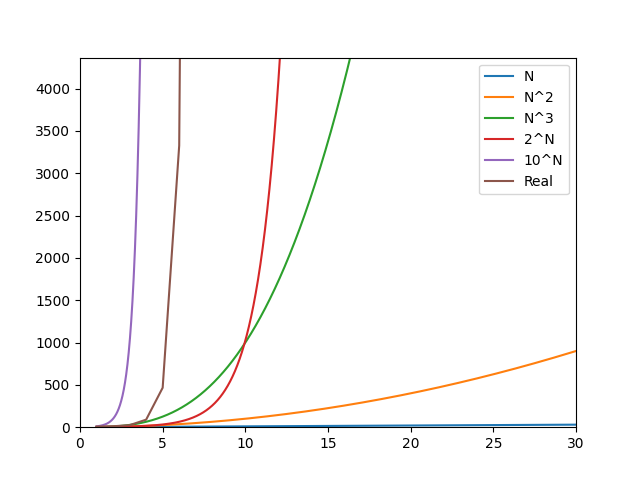
\includegraphics[scale=0.5]{normales.png}%
  \hspace{0.1\linewidth}%
  % Please, notice the use of an optional short caption. 
  \caption[Time vs Input Size (classic version)]{Time vs. Input Size for the non-optimized version of the graph coloring algorithm.}
  \label{fig:res_normales}
\end{figure}

\begin{figure}[p]
  \centering
  % Please, notice the use of comments (%) to avoid extra space.
  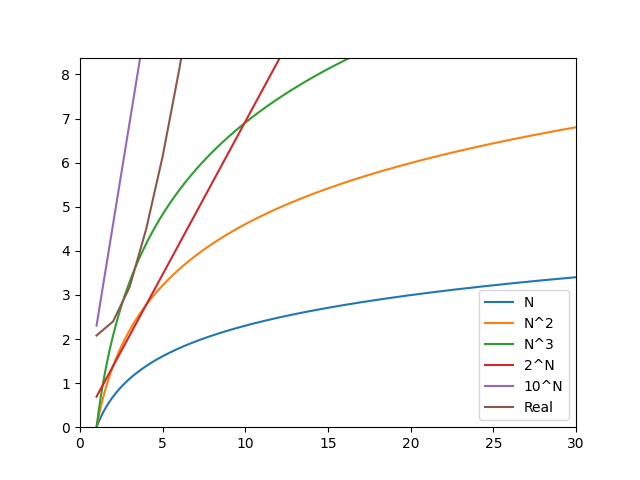
\includegraphics[scale=0.5]{normales_log.png}%
  \hspace{0.1\linewidth}%
  % Please, notice the use of an optional short caption. 
  \caption[Logarithm of Time vs Input Size (classic version)]{Logarithm of Time vs. Input Size for the non-optimized version of the graph coloring algorithm.}
  \label{fig:res_normales_log}
\end{figure}

\begin{figure}[p]
  \centering
  % Please, notice the use of comments (%) to avoid extra space.
  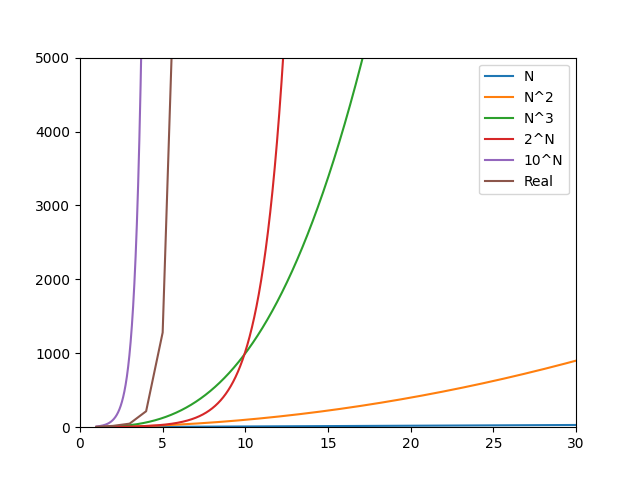
\includegraphics[scale=0.5]{optimizado.png}%
  \hspace{0.1\linewidth}%
  % Please, notice the use of an optional short caption. 
  \caption[Time vs Input Size (optimized version)]{Time vs. Input Size for the optimized version of the graph coloring algorithm.}
  \label{fig:res_optimizado}
\end{figure}

\begin{figure}[p]
  \centering
  % Please, notice the use of comments (%) to avoid extra space.
  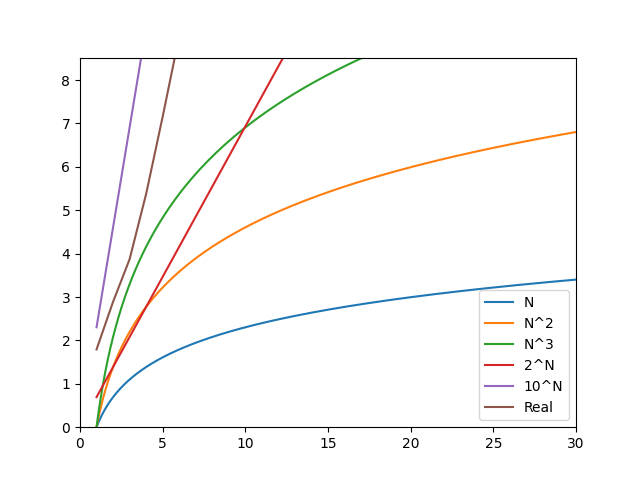
\includegraphics[scale=0.5]{optimizado_log.png}%
  \hspace{0.1\linewidth}%
  % Please, notice the use of an optional short caption. 
  \caption[Logarithm of Time vs Input Size (optimized version)]{Logarithm of Time vs. Input Size for the optimized version of the graph coloring algorithm.}
  \label{fig:res_optimizado_log}
\end{figure}

\clearpage

%%%% CONCLUSIONS %%%%%%%%%%%%%%%%%%%%%%%%%%%%%%%%%%%%%%%%%%%%%%%%%%%%%%%%%%%%%%%

\section{Conclusions}
\label{sec:conclusions}
The algorithm in pseudocode is easy to understand once you examine it closely, although it may take a bit of effort to grasp initially. The implementation in \emph{C++} did pose some challenges for me (especially when dealing with pointers), but I was able to address the issues that arose without too much difficulty.
\\
Regarding the problem instance generator, with the numbers presented in class, it is impossible to obtain a non-complete graph. Each and every generated instance has created conflicts with the remaining vertices, causing the algorithm to always be in the worst possible case (having to traverse a greater number of nodes in the search tree).
\\
Also, when calculating the times for each version of the algorithm, I encountered issues due to the amount of time it took for values of $N>12$. That's why I had to limit the input sizes of the algorithm to a lower range to obtain sufficient times for visualizing the approximate shape of the function on a graph.
\\
\\
Even though all the cases studied have led to an almost exhaustive search of the search tree of the problem, it has helped me better understand the challenges of such algorithms that need to perform complete searches in their search tree. Additionally, it has demonstrated how we can solve a real-world problem (closely related to other types of problems from different areas) by reducing the problem to a known one and for which we have an algorithm that can provide a solution.

\clearpage

%%%%  REFEREroach NCES %%%%%%%%%%%%%%%%%%%%%%%%%%%%%%%%%%%%%%%%%%%%%%%%%%%%%%%%%%%%%%%%

%\section{References}
%\label{sec:references}


% Print the references collected in the first segment. No heading, as we have
% already included a numbered section, References, on their own.

%\printbibliography[segment=1,heading=none]


%%%%%%%%%%%%%%%%%%%%%%%%%%%%%%%%%%%%%%%%%%%%%%%%%%%%%%%%%%%%%%%%%%%%%%%%%%%%%%%%
%                                  APPENDICES                                  %
%%%%%%%%%%%%%%%%%%%%%%%%%%%%%%%%%%%%%%%%%%%%%%%%%%%%%%%%%%%%%%%%%%%%%%%%%%%%%%%% 

%%%%%%%%%%%%%%%%%%%%%%%%%%%%%%%%%%%%%%%%%%%%%%%%%%%%%%%%%%%%%%%%%%%%%%%%%%%%%%%%
%                                 BACK MATTER                                  %
%%%%%%%%%%%%%%%%%%%%%%%%%%%%%%%%%%%%%%%%%%%%%%%%%%%%%%%%%%%%%%%%%%%%%%%%%%%%%%%% 

% In standard classes, the following command is just markup (no visual effect).

% \backmatter

% Instead, we will start a new page after flushing floats.

\cleardoublepage

%%%% BIBLIOGRAPHY %%%%%%%%%%%%%%%%%%%%%%%%%%%%%%%%%%%%%%%%%%%%%%%%%%%%%%%%%%%%%%

\section*{Bibliography}
\label{sec:bibliography}

% Provide some space between the text and the list of references. We can also
% use a small space (\smallskip), a medium one (\medskip), or simply omit it.

\bigskip

% We can comment the following two lines and have just one section: the default
% section, 0. Previously defined segments would then refer to the default
% section and their numeric labels would match those in the following full list
% of references (the bibliography), instead of being independent.

\endrefsection               % Enclose previous segments in the default section.
\newrefsection               % Create a new section.

% Collect and print all the references in the current section.

\nocite{*}
\printbibliography[heading=none]

% With an explicit title:
% 
% \printbibliography[title=Bibliography]

% With the default title in the table of contents:
% 
% \printbibliography[heading=bibintoc]

\end{document}

%%%%%%%%%%%%%%%%%%%%%%%%%%%%%%%%%%%%%%%%%%%%%%%%%%%%%%%%%%%%%%%%%%%%%%%%%%%%%%%%
%
% Emacs related stuff.
%
% Emacs is an incredibly powerful programmable text editor. Please, find
% relevant information in the following links:
%
%     https://www.gnu.org/software/emacs/emacs.html
%     https://www.gnu.org/software/emacs/manual/emacs.html
%
% Emacs' local variables allow to configure Emacs on a per-file basis when a
% file is opened. The following lines are hardly needed, though they will
% not hurt:
%
%     coding: utf-8        ; Coding.
%     mode: latex          ; Major mode for LaTeX.
%     eval: (tex-pdf-mode) ; Minor mode for using PDFLaTeX.
%
% Emacs tries to guess the file encoding automatically. It can even peek the
% file's \usepackage[···]{inputenc} command, if any. The same with the major
% mode for editing LaTeX (latex-mode) and the minor mode for using PDF-TeX/LaTeX
% (tex-pdf-mode) from Emacs. AUCTeX is recommended to everyone willing to use
% Emacs as an integrated development environment for TeX, LaTeX, and
% derivatives.
%
% You may wish to force spell checking of the whole buffer when you finish
% editing your document, be it interactive (M-x ispell-buffer) or not (M-x
% flyspell-buffer).
%
%%%%%%%%%%%%%%%%%%%%%%%%%%%%%%%%%%%%%%%%%%%%%%%%%%%%%%%%%%%%%%%%%%%%%%%%%%%%%%%%

% Local variables:
% eval: (auto-fill-mode)             ; Automatic line breaking.
% fill-column: 80                    ; Last column before line breaking.
% ispell-local-dictionary: "british" ; Dictionary for spell checking.
% eval: (flyspell-mode)              ; Spell checking on the fly.
% End:

